%
% SBXG Design Document
%

\documentclass{article}
\usepackage[T1]{fontenc}
\usepackage[utf8]{inputenc}
\usepackage[english]{babel}

\usepackage{hyperref}
\usepackage{mdframed}
\usepackage{tikz}
\usepackage{thmtools}

\usetikzlibrary{shapes,arrows,positioning}
\tikzstyle{Block} = [draw, rectangle, minimum height=3em, minimum width=3em]
\tikzstyle{Text} = [draw, rectangle]

\newcommand{\email}[1]{%
  \href{mailto:#1}{#1}%
}

\newmdtheoremenv[%
  linecolor=black,
  frametitlerule=true,
]{requirement}{Requirement}

\title{SBXG Design Document}
\date{}
\author{%
  Jean Guyomarc'h%
  \\Jean-Marc Lacroix%
}

\begin{document}

\maketitle
\tableofcontents
\clearpage

\part{Overall description of SBXG}

SBXG is a build orchestrator that provides means to generate from sources or
foreign binaries a ready-to-flash SD (Secure Digital) card image for embedded systems.

SBXG orchestrates several components:
\begin{itemize}
\item a toolchain to compile most of the other components;
\item a bootloader builder;
\item a kernel builder;
\item a kernel packager;
\item an initramfs builder for the kernel that may rely on it;
\item a primary rootfs generator;
\item and a filesystem utility to generate the final image which will contain the
  desired components.
\end{itemize}

All of these components can be used individually, or chained together to
generate more complex systems.



\section{Toolchain Retrieving}

The \emph{toolchain} is a suite of software tools that allows to create another
software. When we refer to a toolchain, we refer to a (cross) compiler driver
and its own components (like gcc and the collection programs it relies on).

Since SBXG is primarily targetting embedded platforms, the toolchain will mostly
be arm-flavoured. The different arm architectures will vary in function of the
\emph{processor} embedded on the SoC that ships with an \emph{embedded board}.

We select our toolchains from \url{https://www.linaro.org/}, but custom ones can
of course be provided.

\begin{requirement}
  SBXG is required to fetch an external toolchain or to use an already existing
  one.
\end{requirement}


\section{Bootloader Builder Component}

The \emph{bootloader} is the piece of software that is responsible for
bootstrapping the primary kernel which will operate the system. In the embedded
world, which consists mainly of ARM-based SoCs, U-Boot is the most prevalent
bootloader. The bootloader builder provided by SBXG is therefore strongly
oriented towards U-Boot.

\begin{center}
  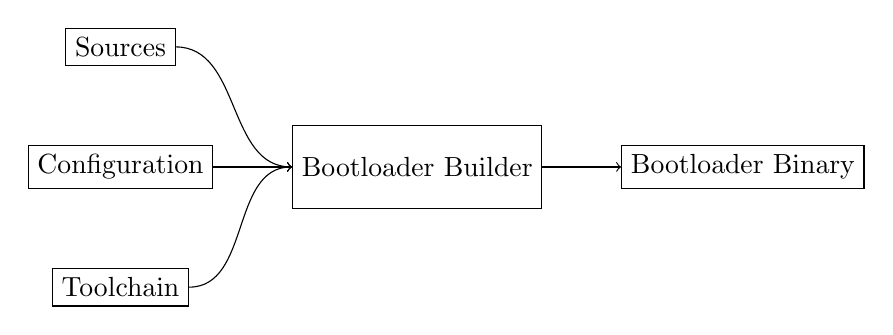
\begin{tikzpicture}
    \node[Block] (component)                      {Bootloader Builder};
    \node[Text]  (config)    [left=of component]  {Configuration};
    \node[Text]  (sources)   [above=of config]    {Sources};
    \node[Text]  (toolchain) [below=of config]    {Toolchain};
    \node[Text]  (output)    [right=of component] {Bootloader Binary};
    \draw[->] (toolchain) to [out=0,in=180] (component);
    \draw[->] (sources)   to [out=0,in=180] (component);
    \draw[->] (config)    to [out=0,in=180] (component);
    \draw[->] (component) to (output);
  \end{tikzpicture}
\end{center}

\begin{requirement}
SBXG is required to generate an U-Boot image.
\end{requirement}


\section{Kernel Components}

The \emph{kernel} is the software that is responsible for user tasks to execute
on a given hardware. We mostly target the Linux kernel, due to its wide range of
drivers, which make it usable on most of the arm SoCs.

Type I hypervisors, such as Xen or Xvisor are also targeted. When considering
hypervisors more generally (type I or type II), guest kernel images shall also
be generated by SBXG.

\begin{requirement}
SBXG is required to generate a Kernel image and associated runtime files.
\end{requirement}

We make the distinction between \emph{kernel building} and \emph{kernel
  packaging}. Kernel building consists in generating raw images from the
sources, whereas kernel packaging consists in generating an archive that
contains kernel products which will be integrated within a package manager.

\subsection{Kernel Builder Component}

\begin{center}
  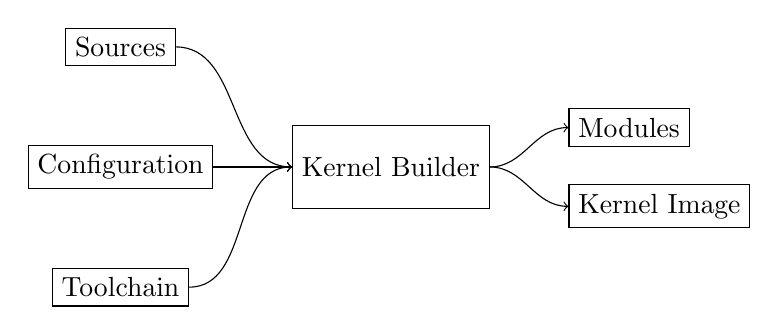
\begin{tikzpicture}
    \node[Block] (component)                      {Kernel Builder};
    \node[Text]  (i_config)    [left=of component]  {Configuration};
    \node[Text]  (i_sources)   [above=of i_config]    {Sources};
    \node[Text]  (i_toolchain) [below=of i_config]    {Toolchain};
    \node[Text]  (o_image)     [right=of component, yshift=-5mm] {Kernel Image};
    \node[Text]  (o_runtime)   [right=of component, yshift=+5mm] {Modules};
    \draw[->] (i_toolchain) to [out=0,in=180] (component);
    \draw[->] (i_sources)   to [out=0,in=180] (component);
    \draw[->] (i_config)    to [out=0,in=180] (component);
    \draw[->] (component)   to [out=0,in=180] (o_image);
    \draw[->] (component)   to [out=0,in=180] (o_runtime);
  \end{tikzpicture}
\end{center}


\subsection{Kernel Packager Component}

\begin{center}
  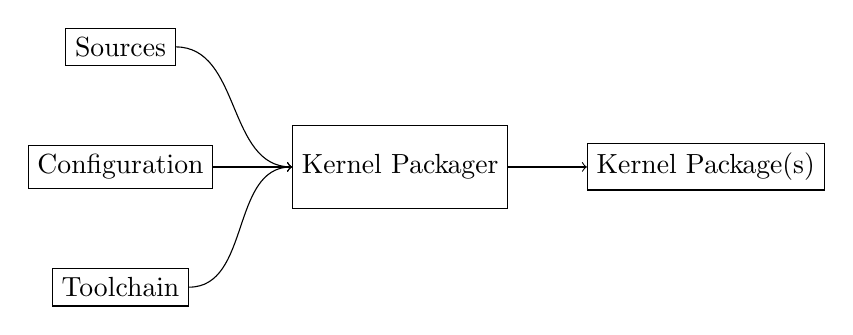
\begin{tikzpicture}
    \node[Block] (component)                        {Kernel Packager};
    \node[Text]  (i_config)    [left=of component]  {Configuration};
    \node[Text]  (i_sources)   [above=of i_config]  {Sources};
    \node[Text]  (i_toolchain) [below=of i_config]  {Toolchain};
    \node[Text]  (o_image)     [right=of component] {Kernel Package(s)};
    \draw[->] (i_toolchain) to [out=0,in=180] (component);
    \draw[->] (i_sources)   to [out=0,in=180] (component);
    \draw[->] (i_config)    to [out=0,in=180] (component);
    \draw[->] (component)   to [out=0,in=180] (o_image);
  \end{tikzpicture}
\end{center}


\section{Initramfs Builder Component}

Some kernels may require an \emph{initramfs} to complete their boot process and
to provide a basic shell in case of failure of the system.

\begin{requirement}
SBXG is required to generate an initramfs on demand. It shall at least support
the CPIO format.
\end{requirement}


\section{Rootfs Generator Component}

The \emph{rootfs} is mounted by the \emph{kernel} and contains the user-land
programs and files that are necessary for the system to operate. Due to the vast
amount of software available, SBXG is not responsible for building a rootfs by
himself. Instead, it shall be able to manipulate an already generated rootfs.

Rootfs can be either build entirely, thanks to software like buildroot or the
Gentoo build system. It can also be retrived as pre-built binaries, thanks to
tools like Deboostrap.

\begin{requirement}
SBXG is required to integrate an externally generated rootfs in its production
pipeline.
\end{requirement}

\section{Description of the execution pipeline}

We define an \emph{execution pipeline} as sequential builds of one or several components.
An execution pipeline can take as inputs:
\begin{itemize}
\item products of previous execution pipelines ;
  \item confi
\end{itemize}

SBXG can produce an \emph{execution pipeline}, which will lead to the creation
of one or several software components. They can be taken as

\end{document}
